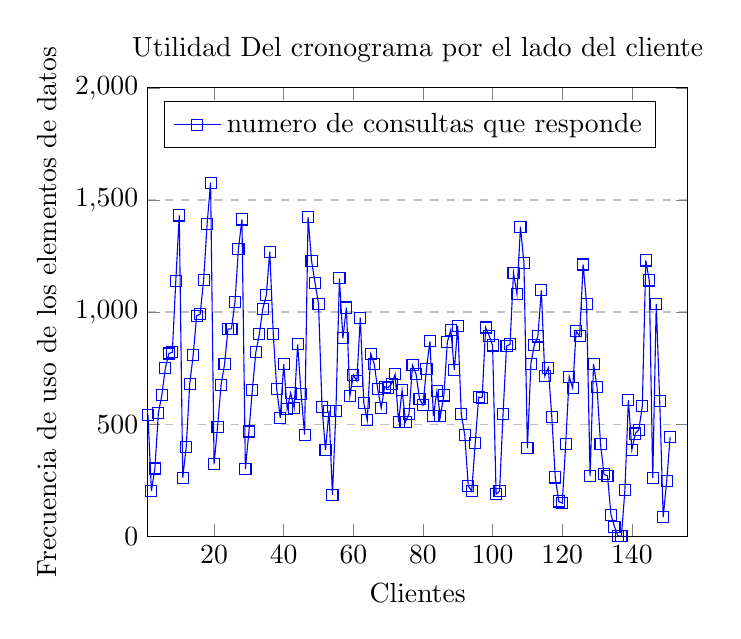
\begin{tikzpicture}
\begin{axis}[
    title={Utilidad Del cronograma por el lado del cliente},
    xlabel={Clientes},
    ylabel={Frecuencia de uso de los elementos de datos},
    xmin=1, xmax=156,
    ymin=0, ymax=2000,
    xtick={},
    ytick={},
    legend pos=north west,
    ymajorgrids=true,
    grid style=dashed,
]

\addplot[
    color=blue,
    mark=square,
    ]
    coordinates {
    %USO EXACTO
    (1,542)
(2,202)
(3,302)
(4,549)
(5,629)
(6,749)
(7,815)
(8,820)
(9,1137)
(10,1431)
(11,261)
(12,399)
(13,678)
(14,808)
(15,984)
(16,990)
(17,1143)
(18,1393)
(19,1577)
(20,321)
(21,488)
(22,674)
(23,767)
(24,924)
(25,925)
(26,1046)
(27,1282)
(28,1413)
(29,299)
(30,467)
(31,654)
(32,821)
(33,902)
(34,1014)
(35,1075)
(36,1269)
(37,902)
(38,656)
(39,528)
(40,767)
(41,567)
(42,639)
(43,573)
(44,856)
(45,635)
(46,453)
(47,1423)
(48,1228)
(49,1130)
(50,1036)
(51,578)
(52,384)
(53,560)
(54,185)
(55,560)
(56,1150)
(57,883)
(58,1020)
(59,625)
(60,719)
(61,693)
(62,975)
(63,595)
(64,517)
(65,813)
(66,768)
(67,656)
(68,572)
(69,667)
(70,663)
(71,680)
(72,722)
(73,509)
(74,651)
(75,511)
(76,546)
(77,762)
(78,724)
(79,613)
(80,584)
(81,746)
(82,869)
(83,536)
(84,646)
(85,535)
(86,628)
(87,866)
(88,921)
(89,741)
(90,938)
(91,545)
(92,451)
(93,225)
(94,201)
(95,414)
(96,620)
(97,618)
(98,931)
(99,894)
(100,851)
(101,187)
(102,201)
(103,545)
(104,848)
(105,856)
(106,1175)
(107,1080)
(108,1381)
(109,1219)
(110,392)
(111,770)
(112,854)
(113,891)
(114,1097)
(115,714)
(116,751)
(117,533)
(118,262)
(119,155)
(120,147)
(121,412)
(122,712)
(123,661)
(124,915)
(125,892)
(126,1212)
(127,1036)
(128,267)
(129,769)
(130,664)
(131,410)
(132,276)
(133,269)
(134,96)
(135,42)
(136,1)
(137,0)
(138,206)
(139,607)
(140,386)
(141,458)
(142,475)
(143,581)
(144,1230)
(145,1141)
(146,259)
(147,1036)
(148,602)
(149,85)
(150,245)
(151,443)
    };
    \legend{numero de consultas que responde}

\end{axis}
\end{tikzpicture}

